\documentclass{report}

\usepackage{fontspec}
\usepackage{geometry}
\usepackage[table]{xcolor}
\usepackage{tabularx}
\usepackage{graphicx}
\usepackage{mathtools}
\usepackage[bottom]{footmisc}
\usepackage[italian]{babel}
\usepackage{hyperref}
\usepackage{titlesec}
\usepackage{listings}
\usepackage{color}
\usepackage{graphicx}

\lstset{ % General setup for the package
    basicstyle=\small\sffamily,
    numbers=left,
     numberstyle=\tiny,
    frame=tb,
    tabsize=4,
    columns=fixed,
    showstringspaces=false,
    showtabs=false,
    keepspaces,
    commentstyle=\color{red},
    keywordstyle=\color{blue}
}

\geometry{
a4paper,
total = {130mm, 240mm},
left = 40mm,
top = 20mm,
}

\setlength{\parindent}{0em}
\setlength{\parskip}{0.7em}

\titlespacing*{\section}{0pt}{0.7em}{0.5em}
\titlespacing*{\subsection}{0pt}{0.7em}{0.5em}

\newcommand{\gassets}{../}


\renewcommand{\title}{
    Analisi dei requisiti
    
    \tiny Versione documento: \textit{V0.0.3}
}

\newcommand{\people}{
    \normalsize
    \begin{center}
        \begin{tabularx}{7cm}{l | X}
            \textbf{Uso} & Esterno\\
            \textbf{Destinatario} & Committente\\
            & Cliente \\
        \end{tabularx}
    \end{center}
}

\fancypagestyle{plain}{%
    \fancyhead{} % clear all header fields
    \fancyhead[L]{\leftmark}
    \fancyhead[R]{\textit{SWEasabi} \includegraphics[height=30pt]{\gassets global-assets/img/loghi/SWEasabi_compact_logo.png}}
    \fancyfoot{} % clear all footer fields
    \fancyfoot[L]{\thepage}
    \fancyfoot[R]{Analisi dei requisiti}
}

\begin{document}

\pagestyle{fancy}

\fancyhead{} % clear all header fields
\fancyhead[L]{\leftmark}
\fancyhead[R]{\textit{SWEasabi} \includegraphics[height=30pt]{\gassets global-assets/img/loghi/SWEasabi_compact_logo.png}}
\fancyfoot{} % clear all footer fields
\fancyfoot[L]{\thepage}
\fancyfoot[R]{Analisi dei requisiti}


\input{\gassets global-assets/tex/header}
\thispagestyle{empty}
\clearpage
\pagenumbering{Roman}
\section{Registro delle modifiche}

\newcommand{\pzerozerouno}{
    \begin{center}
        \begin{tabularx}{\linewidth}{l | X}            
            \textbf{Approvazione} & Peron Samuel\\
            \hline
            \textbf{Redazione} & Bonavigo Michele\\
            & Casarotto Mattia \\
            & Massarenti Alessandro\\
            & Romano Davide \\
            & Zarantonello Giorgio \\
            \hline
            \textbf{Verifica} & Bonavigo Michele\\
            & Massarenti Alessandro\\
            & Pierobon Luca\\
        \end{tabularx}
    \end{center}
}

\newcommand{\vzerozerouno}{
    \hline
    0.0.1 & 16 nov 2022 &  Aggiunta draft dei casi d'uso & \pzerozerouno\\
}

\newcommand{\pzerozerodue}{
    \begin{center}
        \begin{tabularx}{\linewidth}{l | X}            
            \textbf{Approvazione} & Casarotto Mattia\\
            \hline
            \textbf{Redazione} & Massarenti Alessandro\\
            \hline
            \textbf{Verifica} & Bonavigo Michele\\\\
        \end{tabularx}
    \end{center}
}

\newcommand{\vzerozerodue}{
    \hline
    0.0.2 & 30 nov 2022 & Riportata draft delle user stories stesa precedentemente & \pzerozerodue \\
}
\newcommand{\pzerozerotre}{
    \begin{center}
        \begin{tabularx}{\linewidth}{l | X}            
            \textbf{Approvazione} & Casarotto Mattia\\
            \hline
            \textbf{Redazione} & Massarenti Alessandro\\
            & Peron Samuel\\
            & Romano Davide\\
            & Zarantonello Giorgio\\
            \hline
            \textbf{Verifica} & Bonavigo Michele\\\\
        \end{tabularx}
    \end{center}
}

\newcommand{\mzerozerotre}{
    \begin{itemize}
        \item Aggiunta sezione descrizione attori
        \item Aggiunta sezione funzionalità
        \item Aggiunta sezione caratteristiche del prodotto
        \item Aggiunta sezione caratteristiche degli utenti
        \item Aggiunta sezione obiettivi del prodotto
        \item Aggiunta sezione vincoli di progettazione
        \item Aggiunte definizioni del glossario
    \end{itemize}
}

\newcommand{\vzerozerotre}{
    \hline
    0.0.3 & 7 dic 2022 & \mzerozerotre & \pzerozerotre\\
}
\newcommand{\pzerozeroquattro}{
    \begin{center}
        \begin{tabularx}{\linewidth}{l | X}
            \textbf{Approvazione} & Bonavigo Michele\\
            \hline
            \textbf{Redazione} & Bonavigo Michele\\
            & Casarotto Mattia\\
            & Massarenti Alessandro\\
            & Zarantonello Giorgio\\
            \hline
            \textbf{Verifica} & Pierobon Luca\\
            &Massarenti Alessandro\\
            &Bonavigo Michele\\
        \end{tabularx}
    \end{center}
}

\newcommand{\mzerozeroquattro}{
    \begin{itemize}
        \item Riordinati e riscritti completamente i casi d'uso
        \item Migliorata la qualità delle immaigni
    \end{itemize}
}

\newcommand{\vzerozeroquattro}{
    \hline
    0.0.4 & 12 feb 2023 & \mzerozeroquattro & \pzerozeroquattro\\
}
\newcommand{\pzerozerocinque}{
    \begin{center}
        \begin{tabularx}{\linewidth}{l | X}
            \textbf{Approvazione} & Massarenti Alessandro\\
            \hline
            \textbf{Redazione} & Casarotto Mattia\\
            & Massarenti Alessandro\\
            \hline
            \textbf{Verifica} & Massarenti Alessandro\\
            & Bonavigo Michele\\
            & Pierobon Luca\\
        \end{tabularx}
    \end{center}
}

\newcommand{\mzerozerocinque}{
    \begin{itemize}
        \item Correzioni minori su terminologia
        \item Inserita sezione requisiti funzionali
        \item Inserita sezione requisiti di qualità
        \item Inserita sezione requisiti di vincolo
    \end{itemize}
}

\newcommand{\vzerozerocinque}{
    \hline
    0.0.5 & 5 mar 2023 & \mzerozerocinque & \pzerozerocinque\\
}

\newcommand{\pzerozerosei}{
    \begin{center}
        \begin{tabularx}{\linewidth}{l | X}
            \textbf{Approvazione} & Massarenti Alessandro\\
            \hline
            \textbf{Redazione} & Bonavigo Michele \\
            & Massarenti Alessandro\\
            \hline
            \textbf{Verifica} & Pierobon Luca\\
        \end{tabularx}
    \end{center}
}

\newcommand{\mzerozerosei}{
    \begin{itemize}
        \item Aggiunto UC27 per soddisfare il requisito \textbf{RF\_09}
        \item correzioni minori all'immagine dell'UC05
        \item correzioni minori all'immagine dell'applicazione,gestione
    \end{itemize}
}

\newcommand{\vzerozerosei}{
    \hline
    0.0.6 & 7 mar 2023 & \mzerozerosei & \pzerozerosei\\
}

\newcommand{\pzerounozero}{
    \begin{center}
        \begin{tabularx}{\linewidth}{l | X}
            %\textbf{Approvazione} & \\
            % \hline
            % \textbf{Redazione} &  \\
            % \hline
            \textbf{Verifica} & Pierobon Luca\\
        \end{tabularx}
    \end{center}
}

\newcommand{\mzerounozero}{
    \begin{itemize}
        \item Revisione del documento
    \end{itemize}
}

\newcommand{\vzerounozero}{
    \hline
    0.1.0 & 13 mar 2023 & \mzerounozero & \pzerounozero\\
}

\newcommand{\pzerounouno}{
    \begin{center}
        \begin{tabularx}{\linewidth}{l | X}
            \textbf{Approvazione} & Massarenti Alessandro \\
             \hline
             \textbf{Redazione} & Bonavigo Michele \\
             \hline
            \textbf{Verifica} & Pierobon Luca \\
        \end{tabularx}
    \end{center}
}

\newcommand{\mzerounouno}{
    \begin{itemize}
        \item Sistemato un riferimento errato
    \end{itemize}
}

\newcommand{\vzerounouno}{
    \hline
    0.1.1 & 13 mar 2023 & \mzerounouno & \pzerounouno\\
}

\newcommand{\punozerozero}{
    \begin{center}
        \begin{tabularx}{\linewidth}{l | X}
            \textbf{Approvazione} & Massarenti Alessandro\\
            % \hline
            % \textbf{Redazione} &  \\
            % \hline
            % \textbf{Verifica} & \\
        \end{tabularx}
    \end{center}
}

\newcommand{\munozerozero}{
    \begin{itemize}
        \item Approvazione del documento
    \end{itemize}
}

\newcommand{\vunozerozero}{
    \hline
    1.0.0 & 13 mar 2023 & \munozerozero & \punozerozero\\
}


%Tabella
\begin{center}
    \begin{xltabular}{\linewidth}{|l|l|X|X|}
        \hline
        \textbf{Versione} & \textbf{Data} & \textbf{Modifica}& \textbf{Persone}\\
        
        \vunozerozero
        \vzerounouno
        \vzerounozero
        \vzerozerosei
        \vzerozerocinque
        \vzerozeroquattro
        \vzerozerotre
        \vzerozerodue
        \vzerozerouno
        
        \hline

    \end{xltabular}
\end{center}

\tableofcontents
\clearpage
\pagenumbering{arabic}
\chapter{Introduzione}

\section{Glossario}
Un glossario utile con alcune definizioni per lavorare al progetto al fine di chiarire eventuali termini che possono generare
dubbi interpretativi:
\begin{itemize}
    \item \textbf{Area illuminata:} sottoinsieme degli impianti di illuminazione che vengono gestiti in
modo uniforme per intensita' luminosa. Un'area illuminata e' composta da un certo numero di lampioni ed e' dotata di un sensore 
di luminosita' e di un sensore di presenza.
    \item \textbf{Lampione:} sistema di illuminazione facente parte di una specifica area illuminata provvedendo a fornire 
    l'illuminazione per una parte dell'area illuminata.
    \item \textbf{Sensore di luminosita':} sensore avente lo scopo di fornire al sistema il valore dell'intensita' luminosa 
    configurato nell'impianto d'illuminazione di riferimento al fine di valutare se apportare variazioni a tale valore.
    \item \textbf{Sensore di presenza:} sensore avente lo scopo di rilevare presenza di persone in un' area illuminata al fine 
    di variare la luminosita' dell'area a cui afferisce.
\end{itemize}
\section{Caratteristiche degli utenti}

Il portale è rivolto ai soli utenti della piattaforma che si sono già registrati e quindi hanno già un ruolo dentro al sistema.
Questi attori, suddivisi in \textit{Utente Gestore} ed \textit{Utente Manutentore}, hanno un ruolo specifico ed accedono a diverse funzionalità del sistema.

\paragraph{Utente gestore:} La realtà dell'utente gestore è quella di un utente, con il ruolo di impostazione dei valori assegnati alle varie entità disponibili nella piattaforma.

\paragraph{Utente manutentore:} La realtà dell'utente manutentore è quella di un utente, con il ruolo di gestione e manutenzione dei componenti del sistema, con i seguenti compiti:

Esiste inoltre, la figura di \textit{Utente Non Autenticato}, con l'unica scelta di potersi autenticare, per poi ricoprire il ruolo predefinito.

\paragraph{Utente non autenticato:} La realtà dell'utente non autenticato è quella di un utente che non ha ancora fatto il processo di autenticazione, quindi non ha ancora un ruolo definito. La sua unica scelta operativa è l'autenticazione.

\chapter{User stories}

\section{Attori}\label{attori}

\section{Storie utente non loggato}

\begin{itemize}
    \item Utente non loggato può loggarsi
\end{itemize}

\section{Storie utente gestore}

\begin{itemize}
    \item Utente gestore può regolare l'intensità luminosa di un singolo lampione
    \item Utente gestore può regolare l'intensità di molteplici lampioni
    \item Utente gestore può impostare su automatico o manuale l'intensità luminosa di un singolo lampione
    \item Utente gestore può impostare su automatico o manuale l'intensità luminosa di un lampione
    \item Utente gestore può emettere un ticket di guasto
\end{itemize}



\section{Storie utente manutentore}
\begin{itemize}
    \item Utente manutentore può creare nuovi account
    \item Utente manutentore può aggiungere al sistema un nuovo lampione
    \item Utente manutentore può aggiungere al sistema un nuovo sensore
    \item Utente manutentore può aggiungere al sistema aree di gestione illuminazione
    \item Utente manutentore può impostare il raggio d'azione dei sensori
\end{itemize}


\section{Storie lampione}
\begin{itemize}
\item Lampione può cambiare la sua luminosità
\item Lampione riceve dal sistema un valore di luminosità e si regola di conseguenza
\item Il sistema traccia l'intensità luminosa di ogni lampione nel tempo
\end{itemize}


\section{Storie sensore guasti}
\begin{itemize}
\item Sensore guasti se rileva un guasto crea un ticket nel sistema di ticketing
\end{itemize}


\section{Storie sensore dati}
\begin{itemize}
\item Sensore dati invia al database il valore dell'intensità luminosa in un determinato momento
\item Sensore dati invia al sistema l'eventuale presenza di entità
\end{itemize}

\section{Storie sistema di ticketing}
\begin{itemize}
\item Sistema di ticketing riceve un ticket
\end{itemize}

\chapter{Casi d'uso}
\section{Attori}
%lista use-cases
\section{UC01 - Login}

%Una breve descrizione dello use case

\subsection{Attore}
\subsection{Precondizioni}
\subsection{Post-condizioni}
\subsection{Scenario principale}
\subsection{Scenario alternativo}
\section{UC02 - Visualizzazione lista aree}\label{uc:02}

\paragraph{Intenzione in contesto} L'attore primario vuole vedere una lista delle varie aree di illuminazione ed il loro stato.

\paragraph{Attore primario} L'attore primario sono l'utente gestore e manutentore.

\paragraph{Precondizioni} L'attore primario è autenticato ed autorizzato dal sistema.

\paragraph{Postcondizioni} L'attore primario vede la lista delle aree.

\paragraph{Scenario principale}

\begin{enumerate}
    \item L'utente richiede la visualizzazione della lista delle aree;
    \item il sistema fornisce la lista delle aree presenti nel sistema.
\end{enumerate}

\begin{figure}[h]
    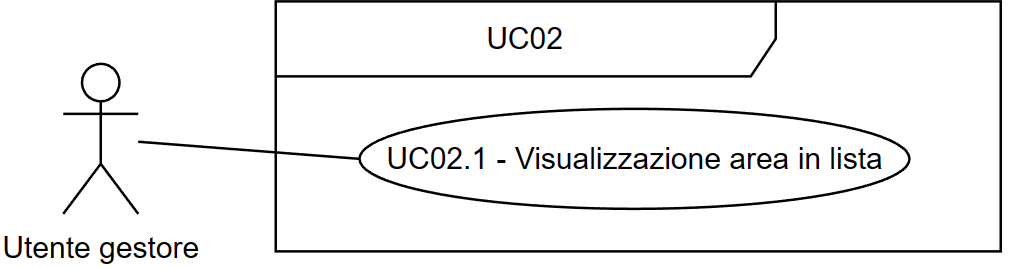
\includegraphics[width=\textwidth]{contenuti/img/casi_uso_grafici-uc02.png}
    \caption{Dettaglio dell'UC02}
    \label{fig:uc02}
\end{figure}

\subsection{UC02.1 Visualizzazione area in lista}
\paragraph{Intenzione in contesto} L'attore primario vuole visualizzare una singola area.

\paragraph{Attore primario} L'attore primario è l'utente gestore.
\paragraph{Precondizioni} L'attore primario è riconosciuto ed autorizzato dal sistema.
\paragraph{Postcondizioni} L'attore primario visualizza la singola area desiderata, in particolare le informazioni relative a \hyperref[uc:02.1.1]{UC02.1.1} e \hyperref[uc:02.1.2]{UC02.1.2}.

\paragraph{Scenario principale}
\begin{enumerate}
    \item L'utente richiede di visualizzare una singola area;
    \item l'utente visualizza la singola area desiderata.
\end{enumerate}

\begin{figure}[h]
    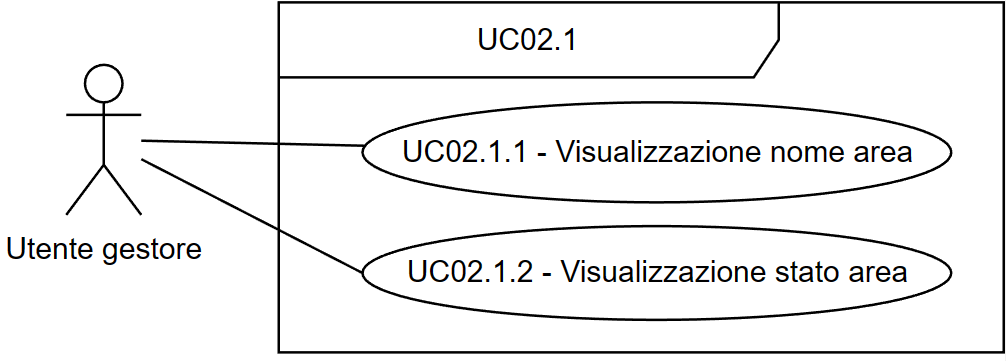
\includegraphics[width=\textwidth]{contenuti/img/casi_uso_grafici-uc02.1.png}
    \caption{Dettaglio dell'UC02.1}
    \label{fig:uc02.1}
\end{figure}

\subsection{UC02.1.1 - Visualizzazione nome area}\label{uc:02.1.1}

\paragraph{Intenzione in contesto} L'attore primario vuole visualizzare il nome dell'area.
\paragraph{Attore primario} L'attore primario è o l'utente gestore o l'utente manutentore.
\paragraph{Precondizioni} L'attore primario è autenticato ed autorizzato dal sistema.
\paragraph{Post-condizioni} L'attore primario visualizza il nome dell'area.
\paragraph{Scenario principale}
\begin{enumerate}
    \item L'attore primario richiede al sistema di visualizzare il nome dell'area;
    \item il nome dell'area è stato visualizzato.
\end{enumerate}

\subsection{UC02.1.2 - Visualizzazione stato area}\label{uc:02.1.2}

\paragraph{Intenzione in contesto} L'attore primario vuole visualizzare lo stato dell'area.
\paragraph{Attore primario} L'attore primario è o l'utente gestore manutentore.
\paragraph{Precondizioni} L'attore primario è autenticato ed autorizzato dal sistema.
\paragraph{Post-condizioni} L'attore primario visualizza lo stato dell'area.
\paragraph{Scenario principale}
\begin{enumerate}
    \item L'attore primario richiede al sistema di visualizzare lo stato dell'area;
    \item lo stato dell'area è stato visualizzato.
\end{enumerate}
\section{UC05 - Visualizzazione dettaglio lampione}\label{uc:05}
\paragraph{Attore primario} L'attore primario è l'utente gestore.
\paragraph{Intenzione in contesto} L'attore primario vuole vedere i dettagli di un lampione, di questo vuole conoscerne lo stato.
\paragraph{Precondizioni}L'attore primario è riconosciuto ed autorizzato dal sistema.
\paragraph{Postcondizioni} L'attore primario visualizza i dettagli e le informazioni su uno specifico lampione.
\paragraph{Scenario principale}
\begin{enumerate}
    \item L'utente richiede di visualizzare i dettagli di uno specifico lampione;
    \item l'utente visualizza i dettagli dello specifico lampione.
\end{enumerate}
\section{UC06 - Aggiunta singolo lampione}

%Una breve descrizione dello use case
\paragraph{Descrizione:}
Come utente installatore/manutentore, voglio aggiungere un singolo lampione al sistema.

\subsection{Attore principale:}
Utente installatore/manutentore.

\subsection{Precondizioni:}
L'utente installatore/manutentore vuole aggiungere al sistema un nuovo lampione.

\subsection{Post-condizioni:}
Il lampione è stato aggiunto al sistema.

\subsection{Scenario principale:}
\begin{enumerate}
    \item L'utente installatore/manutentore inserisce i dati relativi al nuovo lampione;
    \item Il nuovo lampione viene aggiunto al sistema.
\end{enumerate}

\subsection{Scenario alternativo:}
\begin{enumerate}
    \item L'utente installatore/manutentore inserisce valori non ammissibili e il sistema ritorna un errore.
\end{enumerate}
\section{UC10 - Aggiunta area al sistema}\label{uc:10}
\paragraph{Intenzione in contesto} L'attore principale vuole aggiungere una nuova area di gestione dell'illuminazione.

\paragraph{Attore principale} L'attore principale è l'utente manutentore.

\paragraph{Precondizioni}
L'utente principale è autenticato ed autorizzato e vuole aggiungere un area di gestione illuminazione al sistema.

\paragraph{Post-condizioni}
Una nuova area di gestione è stata creata.

\paragraph{Scenario principale}
\begin{enumerate}
    \item L'attore principale crea la nuova area di gestione, inserendo i dati dell'area;
    \item L'area di gestione viene creata nel sistema.
\end{enumerate}



\end{document}
